\documentclass[12pt, a4paper]{report}
\usepackage[top=1cm, left=1cm, right=1cm]{geometry}

\usepackage[utf8]{inputenc}
\usepackage[russian]{babel}

\usepackage{array}
\newcolumntype{M}[1]{>{\centering\arraybackslash}m{#1}}

\usepackage{hyperref}
\hypersetup{
	colorlinks,
	citecolor=black,
	filecolor=black,
	linkcolor=black,
	urlcolor=black
}

\usepackage{sectsty}
\allsectionsfont{\centering}

\usepackage{indentfirst}
\setlength\parindent{24pt}

\usepackage{algorithm}
\usepackage[noend]{algpseudocode}

\usepackage{listings}
\usepackage{xcolor}
\definecolor{codegreen}{rgb}{0,0.6,0}
\definecolor{codegray}{rgb}{0.5,0.5,0.5}
\definecolor{codepurple}{rgb}{0.58,0,0.82}
\definecolor{backcolour}{rgb}{0.95,0.95,0.92}
\lstdefinestyle{mystyle}{
    backgroundcolor=\color{backcolour},
    commentstyle=\color{codegreen},
    keywordstyle=\color{magenta},
    numberstyle=\normalsize\color{codegray},
    stringstyle=\color{codepurple},
    basicstyle=\ttfamily\footnotesize,
    breakatwhitespace=false,
    breaklines=true,
    captionpos=b,
    keepspaces=true,
    numbers=left,
    numbersep=5pt,
    showspaces=false,
    showstringspaces=false,
    showtabs=false,
    tabsize=2
}

\usepackage{graphicx}
\graphicspath{ {plots/pictures/}{assets/pictures} }

\begin{document}
	\begin{titlepage}
		\begin{center}
			\large \textbf{Министерство науки и высшего образования Российской Федерации} \\
			\large \textbf{Федеральное государственное бюджетное образовательное учреждение высшего образования} \\
			\large \textbf{«Российский химико-технологический университет имени Д.И. Менделеева»} \\

			\vspace*{4cm}
			\LARGE \textbf{ОТЧЕТ ПО ЛАБОРАТОРНОЙ РАБОТЕ №6}

			\vspace*{4cm}
			\begin{flushright}
				\Large
				\begin{tabular}{>{\raggedleft\arraybackslash}p{9cm} p{10cm}}
					Выполнил студент группы КС-36: & Золотухин А.А. \\
					Ссылка на репозиторий: & https://github.com/ \\
					& MUCTR-IKT-CPP/ \\
					& ZolotukhinAA\_36\_ALG \\
					Принял: & Крашенников Роман Сергеевич \\
					Дата сдачи: & 07.04.2025 \\
				\end{tabular}
			\end{flushright}

			\vspace*{6cm}
			\Large \textbf{Москва \\ 2025}
		\end{center}
	\end{titlepage}

	\tableofcontents
	\thispagestyle{empty}
	\newpage

	\pagenumbering{arabic}

	\section*{Описание задачи}
	\addcontentsline{toc}{section}{Описание задачи}
	\large
	В рамках лабораторной работы необходимо изучить и реализовать \textit{бинарное дерево поиска} и его самобалансирующийся вариант в лице \textit{AVL-дерева}. \par
	Для проверки анализа работы структуры данных требуется провести \underline{10} серий тестов:
	\begin{itemize}
		\item в каждой серии тестов требуется выполнять \underline{20} циклов генерации и операций. При этом первые \underline{10} работают с массивом заполненным случайным образом, во второй половине случаев, массив заполняется в порядке возрастания значений индекса, т.е. является отсортированным по умолчанию;	
		\item требуется создать массив состоящий из \textit{$ 2^{10 + i} $} элементов, где \textit{i} это номер серии;
		\item массив должен быть помещен в оба варианта двоичных деревьев. При этому замеряется время затраченное на всю операцию вставки всего массива;
		\item после заполнения массива, требуется выполнить \underline{1000} операций поиска по обоим вариантам дерева, случайного числа в диапазоне генерируемых значений, замерев время на все \underline{1000} попыток и вычислив время \underline{1} операции поиска;
		\item провести \underline{1000} операций поиска по массиву, замерить требуемое время на все \underline{1000} операций и найти время на \underline{1} операцию;
		\item после, требуется выполнить \underline{1000} операций удаления значений из двоичных деревьев, и замерить время затраченное на все операции, после чего вычислить время на \underline{1} операцию;
		\item после выполнения всех серий тестов, требуется построить графики зависимости времени затрачиваемого на операции вставки, поиска, удаления от количества элементов. При этом требуется разделить графики для отсортированного набора данных и заполненных со случайным распределением. Так же, для операции поиска, требуется так же нанести для сравнения график времени поиска для обычного массива.
	\end{itemize}

	\newpage

	\section*{Описание метода/модели}
	\addcontentsline{toc}{section}{Описание метода/модели}
	\large

	\newpage

	\section*{Выполнение задачи}
	\addcontentsline{toc}{section}{Выполнение задачи}
	Бинарное дерево поиска и AVL-дерево реализованы на языке \textit{C++}. Построение графиков проводились с помощью программы \textit{GNUplot}.

	\newpage
	\vfill

	\begin{figure}[h]
		\centering
		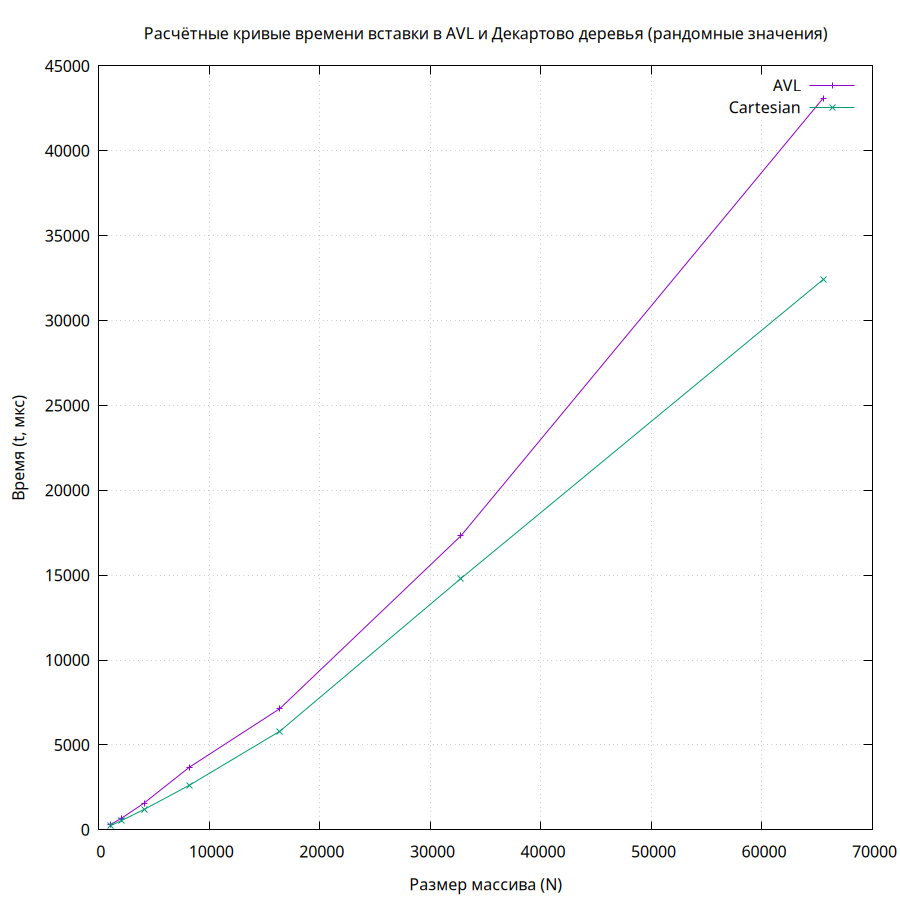
\includegraphics[width=250pt]{insert_random.png}
		\caption{Расчётные кривые времени вставки в BST и AVL деревья (рандомные данные).}
	\end{figure}
	\begin{figure}[h]
		\centering
		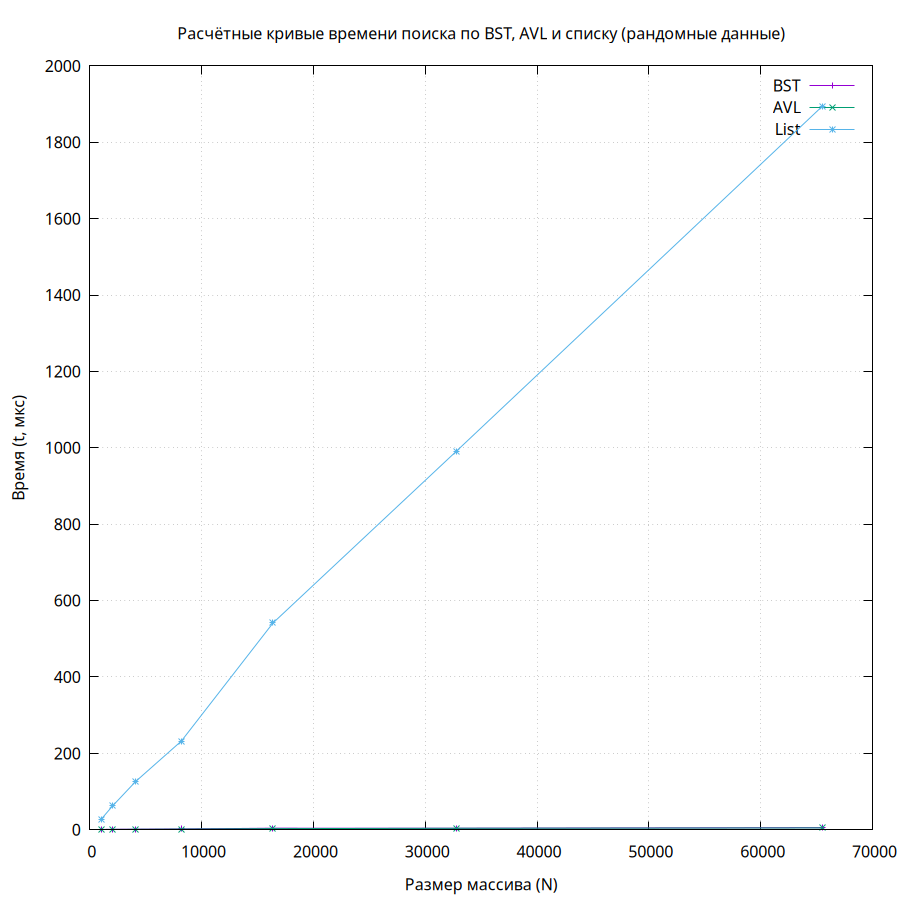
\includegraphics[width=250pt]{search_random.png}
		\caption{Расчётные кривые времени поиска по BST, AVL и списку (рандомные данные).}
	\end{figure}
	\begin{figure}[h]
		\centering
		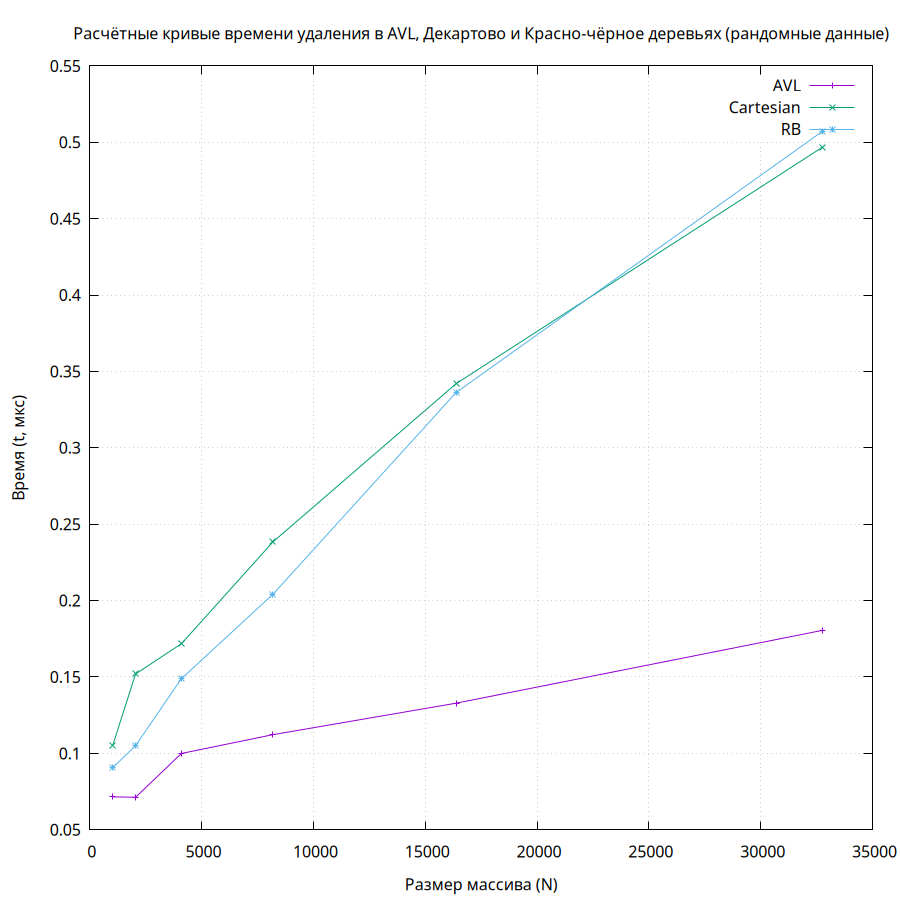
\includegraphics[width=250pt]{delete_random.png}
		\caption{Расчётные кривые времени удаления в BST и AVL деревьях (рандомные данные).}
	\end{figure}
	\begin{figure}[h]
		\centering
		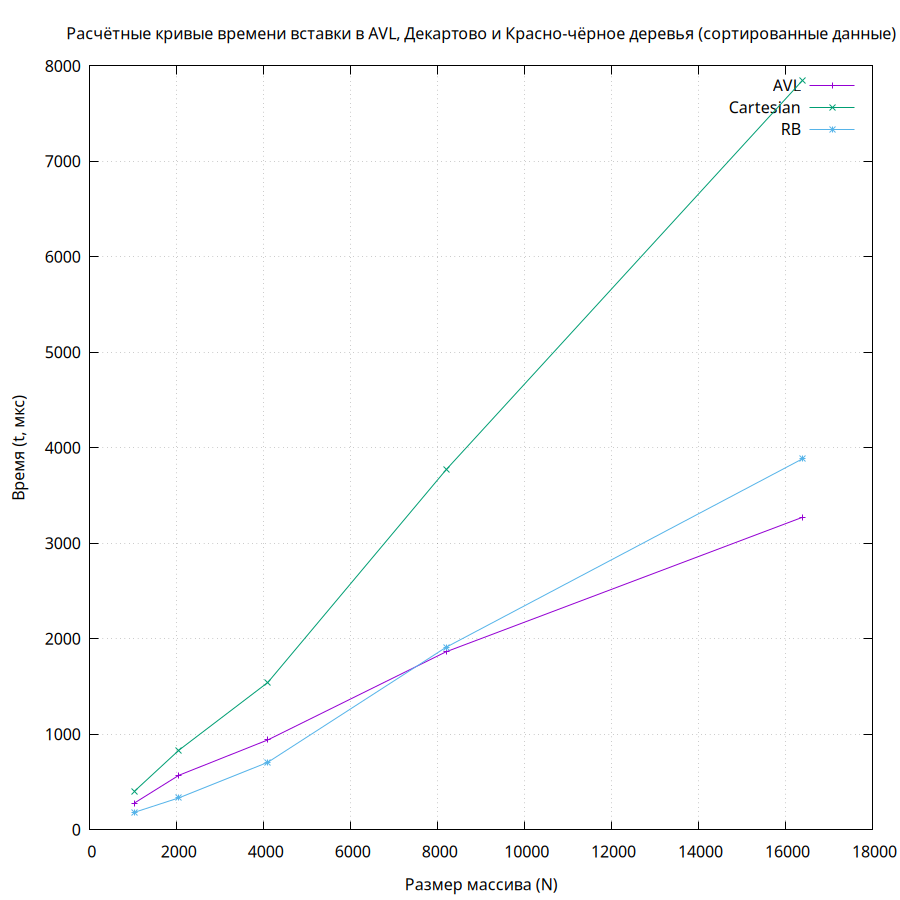
\includegraphics[width=250pt]{insert_sorted.png}
		\caption{Расчётные кривые времени вставки в BST и AVL деревья (сортированные данные).}
	\end{figure}
	\begin{figure}[h]
		\centering
		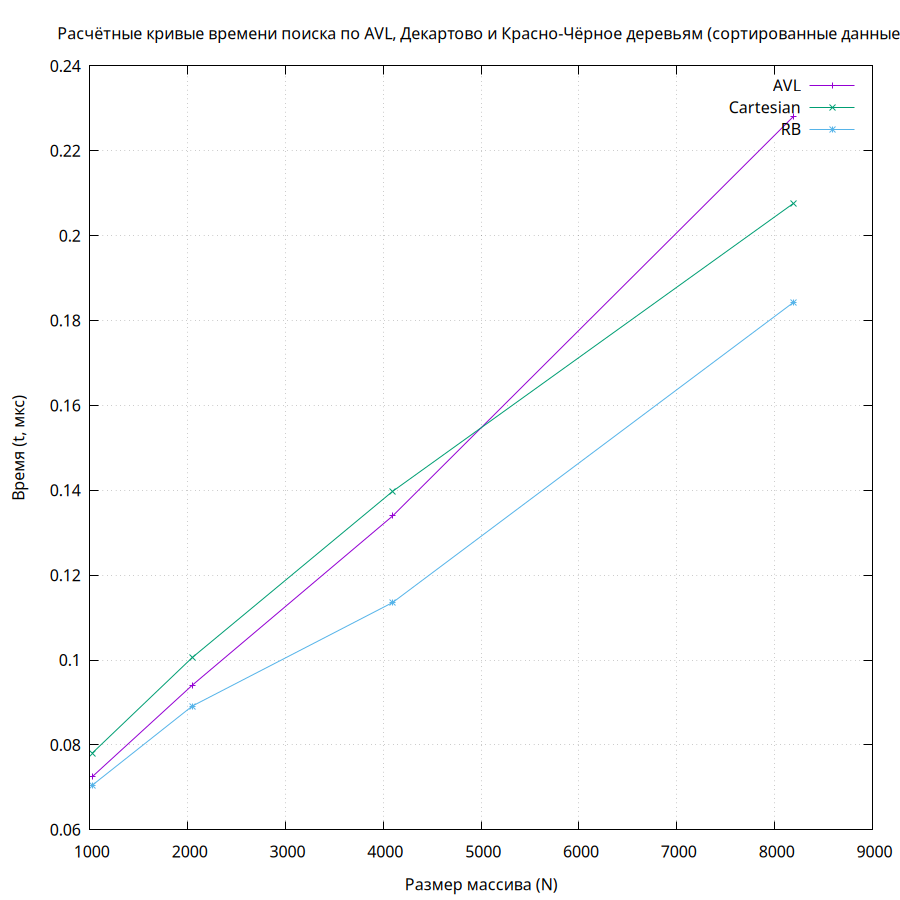
\includegraphics[width=250pt]{search_sorted.png}
		\caption{Расчётные кривые времени поиска по BST, AVL и списку (сортированные данные).}
	\end{figure}
	\begin{figure}[h]
		\centering
		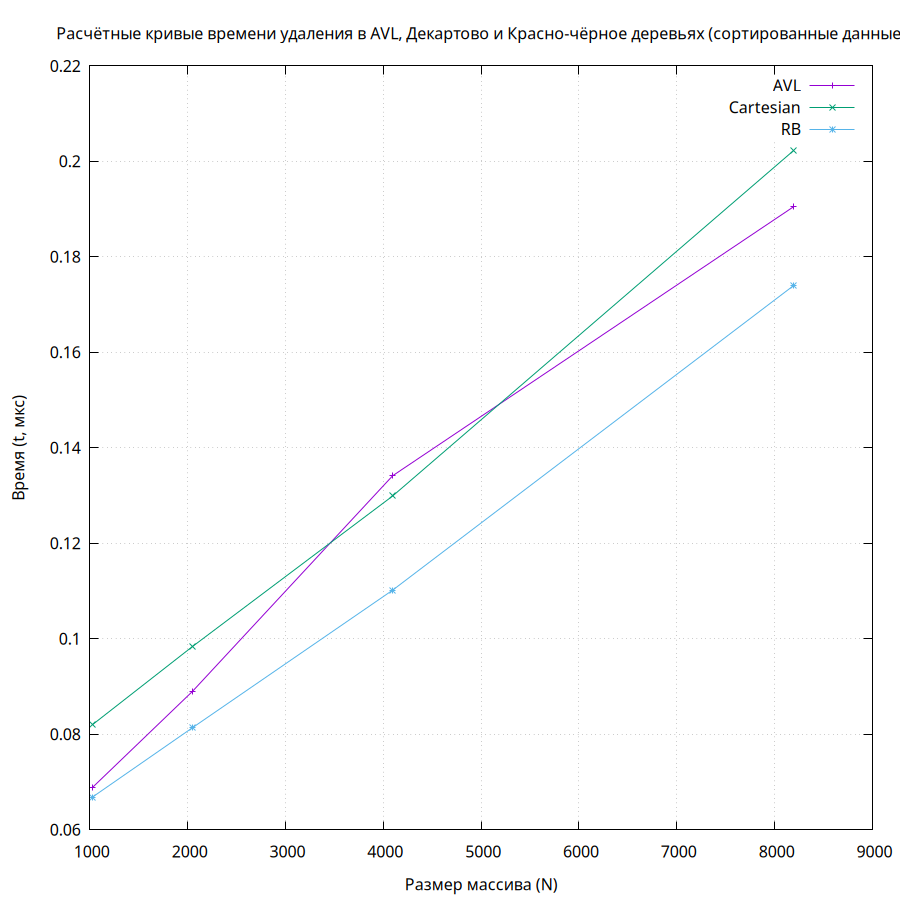
\includegraphics[width=250pt]{delete_sorted.png}
		\caption{Расчётные кривые времени удаления в BST и AVL деревьях (сортированные данные).}
	\end{figure}
\end{document}
